\documentclass[8pt,twocolumn]{article}

\usepackage[a4paper, margin=0.2in]{geometry}
\usepackage{titlesec}
\usepackage{enumitem}
\usepackage{amsmath}
\usepackage{hyperref}
\usepackage{graphicx}
\usepackage{tabularx}
\usepackage{xcolor}
\usepackage{setspace}
\usepackage{listings}  
\usepackage{dsfont}
\usepackage{amssymb}
\usepackage{tikz}
\usetikzlibrary{positioning,arrows.meta}
\newtheorem{theorem}{Theorem}[section]
\newtheorem{lemma}[theorem]{Lemma}
\newtheorem{corollary}[theorem]{Corollary}
\newtheorem{definition}[theorem]{Definition}
\newenvironment{system}%
{\left\lbrace\begin{array}{@{}l@{}}}%
{\end{array}\right.}
\lstset{
  frame=tb,
  language=python,
  aboveskip=2mm,
  belowskip=2mm,
  showstringspaces=false,
  columns=flexible,
  basicstyle={\small\ttfamily},
  keywordstyle=\color{blue}\bfseries,       % <<<< keyword styling
  commentstyle=\color{red}\itshape,
  stringstyle=\color{orange},
  numbers=none,
  breaklines=true,
  breakatwhitespace=true,
  tabsize=3,
  % If you want to highlight extra words:
  morekeywords={} % add your own identifiers here
}
\begin{document}
\makeatletter
\renewcommand\maketitle{%
  \twocolumn[%
    \begin{center}
      \begin{minipage}{0.6\textwidth}  % <-- adjust this width
        \centering
        {\LARGE\bfseries\@title\par}
        {\large\@author\par}
        \vspace{1em}
      \end{minipage}
    \end{center}
  ]
}
\makeatother

\title{CS2109S Final Cheatsheet}
\author{@Wxy2003-xy}
\date{}

\maketitle
\setstretch{0.2}
\setlength{\extrarowheight}{0pt}
\setlength{\parskip}{0pt}
\begin{tabular}{|l|c|c|c|c|}
    \hline
    \textbf{Search} & \textbf{Time} & \textbf{Space} & \textbf{Complete?} & \textbf{Optimal?} \\
    \hline
    BFS  & Exp & Exp  & Yes  & Yes  \\
    UCS  & Exp & Exp  & Yes  & Yes  \\
    DFS  & Exp & Poly & No   & No   \\
    DLS(D)  & Exp & Poly & No   & No   \\
    DLS(B)  & Exp & Exp & No   & Yes   \\
    IDS(D)  & Exp & Exp  & Yes  & Yes  \\
    IDS(B)  & Exp & Exp  & Yes  & Yes  \\
    \hline
\end{tabular}
\newline
\textbf{Informed Search:} Uses heuristics.
\vspace{-0.6em}
\begin{itemize}
    \setlength{\itemsep}{0pt}
    \setlength{\parskip}{0pt}
    \item \textbf{A*}: $f(n) = g(n) + h(n)$.
    \item \textbf{Hill Climbing}: Greedy local search.
\end{itemize}
\vspace{-0.6em}
\vspace{-0.6em}
\begin{itemize}
    \setlength{\itemsep}{0pt}
    \setlength{\parskip}{0pt}
    \item \textbf{Admissibility:} $h(n) \leq h^*(n)$. Never overestimates cost.
    \item \textbf{Consistency:} $h(n) \leq h(n') + c(n, n')$. Guarantees optimality. Implies admissibility
    \item \textbf{Dominance:} $\forall n, h_1(n) \geq h_2(n) \implies h_1$ dominates $h_2$
\end{itemize}
\vspace{-0.6em}
\textbf{Adversarial Search:}
\textbf{Minimax Algorithm:}
\begin{align*}
    \text{max-value}(s) &= \max \text{min-value}(s') \\
    \text{min-value}(s) &= \min \text{max-value}(s')
\end{align*}
\textbf{Alpha-beta pruning:}\vspace{-0.6em}
\begin{lstlisting}[mathescape=true]
    max_value(state, $\alpha$, $\beta$):
        if is_terminal(state): return utility(state)
        v = -$\infty$
        for next_state in expand(state):
            v = max(v, min(v, $\alpha$, $\beta$))
        return v
    
    min_value(state, $\alpha$, $\beta$):
        if is_terminal(state): return utility(state)
        v = $\infty$
        for next_state in expand(state):
            v = min(v, max(v, $\alpha$, $\beta$))
        return v

    alpha-beta search(state): 
        v = max_value(state, -$\infty$, $\infty$) 
        // initialized $\alpha$ to be -$\infty$, $\beta$ to $\infty$
        return action in expand(state) with value v
\end{lstlisting}\vspace{-0.6em}
\textbf{Supervised Learning:} Learns from labeled data.\\
\textbf{Unsupervised Learning:} Finds patterns in unlabeled data.\\
\textbf{Reinforcement Learning:} Learns via rewards.
\textbf{Regression}\\
\textbf{Linear Model:} $h_w(x) = w^T x$. \vspace{-0.6em}
\begin{itemize}
    \setlength{\itemsep}{0pt}
    \setlength{\parskip}{0pt}
    \item \textbf{MSE (L\textsubscript{2})} \vspace{-0.6em}
      \begin{itemize}
        \setlength{\itemsep}{0pt}
        \setlength{\parskip}{0pt}
        \item Definition: \(\frac{1}{n}\sum_{i=1}^n (y_i - \hat y_i)^2\)
        \item Sensitivity to Outliers: squares residuals → heavily penalizes large errors; very sensitive
        \item Differentiability: smooth everywhere; gradient = \(-2(y_i-\hat y_i)\)
        \item Closed‐form Solution: yes (normal equations)
        \item Statistical Interpretation: estimates the conditional \emph{mean} under Gaussian‐noise assumption
        \item Typical Use Cases: Gaussian error models, smooth fast‐converging gradient methods
      \end{itemize}
    \item \textbf{MAE (L\textsubscript{1})} \vspace{-0.6em}
      \begin{itemize}
        \setlength{\itemsep}{0pt}
        \setlength{\parskip}{0pt}
        \item Definition: \(\frac{1}{n}\sum_{i=1}^n \lvert y_i - \hat y_i\rvert\)
        \item Sensitivity to Outliers: linear growth → penalizes proportionally; more robust
        \item Differentiability: not differentiable at zero residual; subgradient = \(\pm1\) elsewhere
        \item Closed‐form Solution: no (requires iterative optimization, e.g. subgradient methods)
        \item Statistical Interpretation: estimates the conditional \emph{median}, robust to heavy tails
        \item Typical Use Cases: heavy‐tailed or outlier‐prone data, when robustness is critical
      \end{itemize}
  \end{itemize}
\textbf{Logistic Regression}\\
\textbf{Sigmoid Function:} $\sigma(x) = \frac{1}{1 + e^{-x}}$. \\
\textbf{(BCE) Binary Cross Entropy Loss:}
\begin{equation}
    BCE(y, \hat{y}) = -y\log(\hat{y}) - (1 - y)\log(1 - \hat{y})
\end{equation}
\textbf{Loss function:}
\begin{equation}
    \begin{system}
    -log(h_w(x)), \text{ if y = 1}\\
    -log(1 - h_w(x)), \text{if y = 0}
    \end{system}
\end{equation}
\textbf{Gradient Descent:}
\begin{equation}
    w_j \leftarrow w_j - \gamma \frac{\partial J}{\partial w_j}
\end{equation}
    \[\frac{\partial }{\partial w_0} J_{MSE}(w)= \frac{1}{N} \sum_{i=1}^{N}((w_0 + w_1 x^{(i)}) - y^{(i)}) \quad {(x_0 = 1)}\]
    \[\frac{\partial }{\partial w_1} J_{MSE}(w)= \frac{1}{N} \sum_{i=1}^{N}((w_0 + w_1 x^{(i)}) - y^{(i)})(x^{(i)})\]
\textbf{Normal Equation:} $w = (X^TX)^{-1}X^Ty$.\\
\textbf{Gradient Descent}\vspace{-0.6em}
\begin{lstlisting}[mathescape=true]
    def gradient_descent_multi_variable(X, y, lr = 1e-5, number_of_epochs = 250):
        bias:number = 0
        weights = np.full((X.shape[1], 1), 0).astype(float)
        loss:List[number] = []
        N:number = X.shape[0]  
        pred = X @ weights + bias       
# pred:$\mathbb{R}^{m\times 1}$ = $X:\mathbb{R}^{m\times n} \times w:\mathbb{R}^{n\times 1} $+ bias:number
        for e in range(number_of_epochs): 
            pred = X @ weights + bias
            g_w = (1 / N) * (X.T @ (pred - y)) 
# $\frac{\partial }{\partial w_1}J_{MSE}(w) = \frac{1}{N} X^T((Xw + bias) - y)$
            g_b = (1 / N) * np.sum(pred - y)   
# $\frac{\partial }{\partial w_0}J_{MSE}(w) = \frac{1}{N} \sum_{i=1}^{N} ((Xw + bias) - y)$
            bias -= lr * g_b                   
# $w_0 \leftarrow w_0 - \gamma \frac{\partial J_{MSE}(w)}{\partial w_0}$
            weights -= lr * g_w                
# $w_1 \leftarrow w_1 - \gamma \frac{\partial J_{MSE}(w)}{\partial w_1}$
            loss.append(mean_squared_error(y, pred))
        return bias, weights, loss  
    \end{lstlisting}
\vspace{-1.2em}
\begin{itemize}
    \setlength{\itemsep}{0pt}
    \setlength{\parskip}{0pt}
    \item \textbf{L2 Regularization (Ridge)}\vspace{-0.6em}
      \begin{itemize}
        \setlength{\itemsep}{0pt}
        \setlength{\parskip}{0pt}
        \item Penalty: \(\lambda \sum_{i=1}^d w_i^2\)
        \item Effect: Shrinks all weights toward zero but rarely to exactly zero
        \item Geometry: Elliptical constraint region
        \item Closed‐form Solution: Yes, normal equation
        \item Differentiability: Smooth everywhere → easy gradient‐based optimization
        \item Use Cases: Multicollinearity handling; when you want small weights without feature elimination
      \end{itemize}
    \item \textbf{L1 Regularization (Lasso)}\vspace{-0.6em}
      \begin{itemize}
        \setlength{\itemsep}{0pt}
        \setlength{\parskip}{0pt}
        \item Penalty: \(\lambda \sum_{i=1}^d |w_i|\)
        \item Effect: Encourages sparsity; many weights become exactly zero
        \item Geometry: Diamond-shaped constraint region
        \item Closed‐form Solution: No; solved via iterative methods (e.g. coordinate descent)
        \item Differentiability: Non-smooth at zero
        \item Use Cases: Automatic feature selection; sparse model
      \end{itemize}
  \end{itemize}\vspace{-0.6em}
\textbf{Classification Metrics}\vspace{-0.6em}
\begin{itemize}
    \setlength{\itemsep}{0pt}
    \setlength{\parskip}{0pt}
    \item \textbf{Accuracy}: $\frac{TP + TN}{TP + FN + FP + TN}$.
    \item \textbf{Precision}: $\frac{TP}{TP + FP}$.
    \item \textbf{Recall}: $\frac{TP}{TP + FN}$.
    \item \textbf{F1-score}: $\frac{2}{\frac{1}{P} + \frac{1}{R}}$.
\end{itemize}
\vspace{-0.6em}
\textbf{Decision Trees}\vspace{-0.6em}
\begin{lstlisting}[mathescape=true]
    DTL(examples, attributes, default):
        if (examples = $\emptyset$): return default
        if ($\forall e \in example, \text{e has the same classification }c$): return c
        if (attributes = $\emptyset$): return mode(examples)

        best = choose_attribute(attributes, examples)
        tree = new decision tree with root test $best$
        for $v_i$ of $best$ do:
            examples_i = $\{e | e \in examples, e.best = v_i\}$
            subtree = DTL(examples, attributes \ best, 
                          mode(examples))
            tree.add($v_i$: subtree)


    choose_attribute(attributes, examples):
        best_gain = -$\infty$
        best_attr = None
    
        for attr in attributes:
            gain = information_gain(attr, examples)
            if gain > best_gain:
                best_gain = gain
                best_attr = attr
        return best_attr
    \end{lstlisting}\vspace{-0.6em}
    For data set contains boolean outputs, 
    \[I(P(+), P(-)) = -\frac{p}{p + n}log_2 \frac{p}{p + n} - \frac{n}{p+n}log_2\frac{n}{p+n}\]
    where $0 \leq \mathbb{R}_I \leq 1$. However for non-binary variables the entropy can be greater than 1\\
    \textbf{Information gain}
    Information gain = entropy of this node - entropy of children nodes
    \[IG(A) = I(\frac{p}{p + n}, \frac{n}{p + n}) - remainder(A)\] Initial $I = 1$
    \[remainder(A) = \sum_{i=1}^{v}\frac{p_i + n_i}{p + n}I(\frac{p_i}{p_i + n_i}, \frac{n_i}{p_i + n_i})\]
\textbf{Normal equation}:\vspace{-0.6em}
\[w = (X^T X)^{-1} X^T y\]
\textbf{Multiclass Classification:}\\
\textbf{One-vs-One:} Train $C(C-1)/2$ classifiers.\\
\textbf{One-vs-Rest:} Train $C$ classifiers.\\
\textbf{Binary Cross Entropy}
\[BCE(y, \hat{y}) = -ylog(\hat{y}) - (1 - y)log(1 - \hat{y})\]
\[J_{BCE}(w) = \frac{1}{N} \sum_{i=1}^{N} BCE(y^{(i)}, h_w(x^{(i)}))\]
$\sigma(x) = \frac{1}{1 + e^{-x}}$ is Not convex, but
$-log(\sigma(x))$ is convex\\
Hypothesis function
\[h_w(x) = \sigma(w_0, w_1 x_1 + w_2 x_2) \]
Weight Update
\[w_j \leftarrow w_j - \gamma \frac{\partial J_{BCE}(w_0, w_1, \dots)}{\partial w_j}\]
Loss function derivative
\[\frac{\partial J_{BCE}(w_j)}{\partial w} = \frac{1}{N} \sum_{i=1}^{N} (h_w(x^{(i)}) - y^{(i)})x_j^{(i)}\]
\textbf{Feature Transformation}
    Modify the original features of a dataset to make them more suitable for modeling.\vspace{-0.6em}
    \begin{itemize}
        \setlength{\itemsep}{0pt}
        \setlength{\parskip}{0pt}
        \item Feature engineering\vspace{-0.6em}
            \begin{itemize}
                \setlength{\itemsep}{0pt}
                \setlength{\parskip}{0pt}
                \item Polynomial features: $z = x^k, k$ is the polynomial degree.
                \item log feature: $z = \log(x)$
                \item Exp. feature: $z = e^x$
            \end{itemize}
        \item Feature scale \vspace{-0.6em}
            \begin{itemize}
                \setlength{\itemsep}{0pt}
                \setlength{\parskip}{0pt}
                \item Min-max scaling: $z_i = \frac{x_i - min(x_i)}{max(x_i) - min(x-i)}$, scales to [0, 1]
                \item standardization: $z_i = \frac{x_i - \mu_i}{\sigma_i}$, transformed data has mean of 0 and SD of 1
                \item robust scaling (not in syl)
            \end{itemize}
    \end{itemize}\vspace{-0.6em}
\textbf{SVM:} transformed feature vector: $\mathbb{R}^{d} \mapsto \mathbb{R}^{M}$
\[
x = [x_1,\,x_2,\,x_3]^\top
\;\mapsto\;
\phi_{M_2}(x)
= [\,x_1,\,x_2,\,x_3,\,x_1^2,\,x_2^2,\,x_3^2,\,x_1x_2,\,x_1x_3,\,x_2x_3\,]^\top.
\]

\[h^{\phi}_w(x) = w_0\phi(x)_0 + w_1\phi(x)_1 + ... + w_M\phi(x)_M,\quad \phi(x)_0 = 1\]
\[h^{\phi}_w(x) = w^T\phi(x)\]
\textbf{Dual hypothesis:}\\
$h^{\phi}_\alpha(x) = \sum_{j=1}^{N}\alpha_j \phi^T(x^{(j)})\phi(x),$
$\text{let } k_\phi(u, v) = \phi^T(x^{(j)})\phi(x) \implies h^{\phi}_\alpha(x) = \sum_{j=1}^{N}\alpha_j k_\phi(u, v)$\\
For $n$ degree polynomial, $k_{Pn}(u, v) = \phi_{Pn}^T(x^{(j)})\phi_{Pn}(x) = (u^Tv)^n$\\
\textbf{Gaussian kernel:} $k_{RBF}(u, v):= e^{-\frac{||u-v||^2}{2\sigma^2}}$\\
feature map $\phi_{RBF}$ can map to infinite-dim space, cannot be computed explicitly. \\
Small $\sigma^2$: pointy; large $\sigma^2$: flat\\
\textbf{K-means clustering:} K-means relies on Euclidean distance and assumeslinearly separable clusters
\begin{lstlisting}[mathescape = true]
# Initialize K cluster centroids randomly from the dataset
    for k = 1 in K clusters:
        $\mu_k$ = random($x \in D$)   // Pick a random data point x from dataset D as the initial centroid
    
# Repeat until convergence (e.g., centroids stop moving)
    while (! convergence):
# Assignment step: assign each point to the nearest centroid
        for i = 1 in m:
            $c_i$ = $argmin_k||x^{(i)} - \mu_k||^2$   // Assign point $x^{(i)}$ to the closest cluster (minimizing squared distance)
    
# Update step: move centroids to the mean of assigned points
        for k = 1 in K:
            $\displaystyle \mu_k = \frac{1}{|\{x^{(i)} | c^{(i)} = k\}|} \sum_{x\in \{x^{(i)} | c^{(i)} = k\}}^{}x$  
# Recompute centroid $\mu_k$ as the mean of all points assigned to cluster k
    \end{lstlisting}
\textbf{Distortion:}\\
$J(c^{(1)}, c^{(2)}, \dots, c^{(N)}, \boldsymbol{\mu_1}, \boldsymbol{\mu_2}, ..., \boldsymbol{\mu_K}) = \frac{1}{N}\sum_{i=1}^{N}||x^{(i)} - \boldsymbol{\mu_{c^{(i)}}}||$\\
Each step in the K-Means algorithm never increases distortion
\textbf{Mean-centred Data}\\
mean feature vector over $\{x^{(i)}\}$
\textbf{Dimension reducation:}\\
SVD decomp: $A^{d \times N} = U^{d \times d}\Sigma^{d \times N} V^{T {(N \times N)}}$

\begin{theorem}
    given a mean-centred data matrix $\hat{X}^T$, the values $\frac{\sigma_j^2}{N - 1}$ is the variance of the data in the basis defined by the vectors $u^{(j)}$
\end{theorem}
Variance: $V_p[X] = E_p[(X - E_p(X))^2]$\\
Choose minimum r, to explaine $a$ variance 
\[\rightarrow \frac{\sum_{i=1}^{r}\sigma_i^2}{\sum_{i=1}^{N}\sigma_i^2} \geq a 
\rightarrow \text{...} = \frac{\sum_{i=1}^{N}||\hat{x_i}^{(i)} - \tilde{x_i}^{(i)}||^2}{\sum_{i=1}^{N} ||\hat{x}^{(i)}||^2} \leq 1 - a\]
\[\]
\textbf{Principal Component Analysis:}
Statistics application of SVD. Capture components that maximize the statistical variations of the data. Same idea, but uses sample covariance matrix as an input
\begin{itemize}
    \setlength{\itemsep}{0pt}
    \setlength{\parskip}{0pt}
    \item \textbf{Classification}
      \begin{itemize}
        \setlength{\itemsep}{0pt}
        \setlength{\parskip}{0pt}
        \item \textbf{Type of Feedback:} Supervised learning
        \item \textbf{Input:} Input–output pairs \(\{(x^{(i)},y^{(i)})\}\)
        \item \textbf{Output:} Model \(h(x)\to\hat y\)
        \item \textbf{Methods:} Hyperplane‐based (e.g.\ SVM), probability‐based (e.g.\ logistic regression)
        \item \textbf{Number of Classes:} Defined by the dataset
      \end{itemize}
    \item \textbf{Clustering}
      \begin{itemize}
        \setlength{\itemsep}{0pt}
        \setlength{\parskip}{0pt}
        \item \textbf{Type of Feedback:} Unsupervised learning
        \item \textbf{Input:} Data points only \(\{x^{(i)}\}\)
        \item \textbf{Output:} Group assignments (e.g.\ \(x^{(1)}\) → cluster 5)
        \item \textbf{Methods:} Distance‐based algorithms
        \item \textbf{Number of Clusters:} Chosen by practitioner\(^*\)
      \end{itemize}
  \end{itemize}  \vspace{-0.6em}
\textbf{Generalization} \vspace{-0.6em}
\begin{itemize}
    \setlength{\itemsep}{0pt}
    \setlength{\parskip}{0pt}
    \item In supervised learning, and machine learning in general, the model's performance on unseen data is all we care about. This ability to perform well on new, unseen data is known as the model's generalization capability. 
    \item There are two factors that affect generalization:
    \vspace{-0.6em}
    \begin{itemize}
        \setlength{\itemsep}{0pt}
        \setlength{\parskip}{0pt}
        \item Dataset quality \vspace{-0.3em}
        \begin{itemize}
            \setlength{\itemsep}{0pt}
            \setlength{\parskip}{0pt}
            \item Relevance
            \item Noise (irrelevant or incorrect data)
            \item Balance (for classification): Balanced datasets ensure that all classes are adequately represented e.g. ratio
        \end{itemize}
    \vspace{-0.3em}
        \item Data quantity\vspace{-0.3em}
        \begin{itemize}
            \setlength{\itemsep}{0pt}
            \setlength{\parskip}{0pt}
            \item In general, having more data typically leads to better model performance
            \item Extreme case: if the dataset contains every possible data point, memorize
        \end{itemize}
        \vspace{-0.3em}
        \item Model complexity\vspace{-0.3em}
        \begin{itemize}
            \setlength{\itemsep}{0pt}
            \setlength{\parskip}{0pt}
            \item Size and expressiveness of the hypothesis class.
            \item Intricacy of the relationships between input and output variables that the model can capture.
        \end{itemize}
    \end{itemize}
\end{itemize} \vspace{-0.6em}
\textbf{Hyperparameter}
Hyperparameters are settings that control the behavior of the training algorithm and model but are not learned from the data. They need to be set before the training process begins. Such as \vspace{-0.6em}
\begin{itemize}
    \setlength{\itemsep}{0pt}
    \setlength{\parskip}{0pt}
    \item Learning rate
    \item Feature transformations
    \item Batch size and iterations in mini-batch gradient descent
\end{itemize}\vspace{-0.6em}
\textbf{Perceptron Learning algorithm:}\vspace{-0.6em}
\begin{lstlisting}[mathescape = true]
initialize $\textbf{w}$
while (i < max_iteration | !convergence):
    for ($x_i$, $y_i$) in D:
        $\hat{y} = h_w(x)$
        if $x_i$ is misclassified:
            learning_error = $(y_i - \hat{y}_i)$
            w += $\gamma (y_i - \hat{y}_i) x_i$
\end{lstlisting}\vspace{-0.6em}
On data not linearly separable The algorithm will not converge
    \[\hat{y} = sgn(\textbf{w}^Tx)\]
Case 1: $y = +1, \hat{y} = -1$: $\hat{y} < 1 \implies \textbf{w}^Tx < 0 \implies \textbf{w}x < 0 \implies |\textbf{w}||x|\cos\theta < 0 \implies \theta \in (\frac{\pi}{2}, \pi)$\\
\indent But we want the opposite, ie $\hat{y} = +1 \implies \theta \in [0, \frac{\pi}{2}] \implies$ Reduce $\theta$\\
\indent $\textbf{w}' = \textbf{w} + x \implies \theta' < \theta$ \\
Case 2: $y = -1, \hat{y} = +1$ Similarly, $\textbf{w}' = \textbf{w} - x \implies \theta' > \theta$\\
\[\textbf{w}' \leftarrow \textbf{w} + 2\gamma x, \textbf{w}' \leftarrow \textbf{w} + \gamma(+1 - (-1)) x \]
\[\textbf{w}' \leftarrow \textbf{w} + \gamma(y - \hat{y}) x \]
Trivial to show, both cases arrive at the same update rule.\\
\textbf{Multilayer neural network:}
Single-layer NN is equivalent to a linear classifier\vspace{-0.6em}
\begin{itemize}
    \setlength{\itemsep}{0pt}
    \setlength{\parskip}{0pt}
    \item \textbf{Depth (number of hidden layers $L$)} complexity grows roughly $\mathcal{O}(L)$ in layers.
    \item \textbf{Width (number of input features $d$)} per‐layer cost grows roughly $\mathcal{O}(d)$ (or $\mathcal{O}(d\cdot n)$ if hidden size is $n$).
  \end{itemize}\vspace{-0.6em}
\[\textbf{x} = \begin{bmatrix}
    x_1 \\ x_2\\x_3
    \end{bmatrix}, \textbf{W}^{[1]} = \begin{bmatrix}
        W^{[1]}_{11} & W^{[1]}_{12} \\ W^{[1]}_{21} & W^{[1]}_{22}\\ W^{[1]}_{31} & W^{[1]}_{32} 
        \end{bmatrix}\]
        \[\hat{y}^{[1]} = g^{[1]}(\textbf{W}^{[1]T}x)\]
\textbf{Forward Propagation:} For n layers, 
\[\hat{y}^{[n]} = g^{[n]}(W^{[n]^T}\hat{y}^{[n-1]})\]
\[\hat{y} = g^{[n]}(W^{[n]^T}(g^{[n-1]}(W^{[n-1]^T}... g^{[2]}(W^{[2]^T} g^{[1]}(W^{[1]^T}\textbf{x})))))\]
Example:
\[
\mathbf{x} = \begin{bmatrix}
  x_1 \\ x_2 \\ x_3
\end{bmatrix}, 
\mathbf{W}^{[1]} = \begin{bmatrix}
  W^{[1]}_{11} & W^{[1]}_{12} & W^{[1]}_{13} \\
  W^{[1]}_{21} & W^{[1]}_{22} & W^{[1]}_{23} \\
  W^{[1]}_{31} & W^{[1]}_{32} & W^{[1]}_{33}
\end{bmatrix}, 
\mathbf{W}^{[2]} = \begin{bmatrix}
  W^{[2]}_{11} & W^{[2]}_{12} \\
  W^{[2]}_{21} & W^{[2]}_{22} \\
  W^{[2]}_{31} & W^{[2]}_{32}
\end{bmatrix}
\]
\[
\hat{\mathbf{y}}^{[1]}
= g^{[1]}\bigl(\mathbf{W}^{[1]\!T}\,\mathbf{x}\bigr),
\qquad
\hat{\mathbf{y}}
= g^{[2]}\bigl(\mathbf{W}^{[2]\!T}\,\hat{\mathbf{y}}^{[1]}\bigr)
= \begin{bmatrix} \hat y_1 \\ \hat y_2 \end{bmatrix}.
\]
\textbf{Multi class classification}
Softmax function
\[\textbf{x}^{N\times 1} \rightarrow \textbf{z}^{C \times 1}\]
$\forall z_i \in \textbf{z}, i \in [1, C], z_i \in [0, 1]$, as $z_i$ indicates the probability of $\textbf{x}$ belonging to class $C_i$. 
To map the neuron network output from $\mathbb{R}$ to $[0, 1]$, we use softmax function: 
\[g(z_i) = \frac{e^{z_i}}{\sum_{i=1}^{C} z_i}\]
where $\mathbb{R}_g = [0, 1]$, and $\sum_{i=1}^{C} g(z_i) = 1$, indicating a complete probability distributon.\\
\textbf{Chain rule:}
\[l = h(g(f(x))) \xrightarrow{\text{deriv.}} \frac{\partial l}{\partial x} 
= \frac{\partial l}{\partial y}\frac{\partial y}{\partial z}\frac{\partial z}{\partial x}\]
where $z = f(x), y = g(z), l = h(y)$\\
\textbf{Backpropagation:}
\[
\begin{aligned}
\mathbf{z}^{[1]} &= \mathbf{W}^{[1]\!T}\,\mathbf{x}, 
&\quad
\mathbf{a}^{[1]} &= g^{[1]}\bigl(\mathbf{z}^{[1]}\bigr),\\
\mathbf{z}^{[2]} &= \mathbf{W}^{[2]\!T}\,\mathbf{a}^{[1]}, 
&\quad
\hat{\mathbf{y}} &= g^{[2]}\bigl(\mathbf{z}^{[2]}\bigr).
\end{aligned}
\]
\[
\hat{\mathbf{y}}
= g^{[2]}\Bigl(\mathbf{W}^{[2]\!T}\;g^{[1]}\bigl(\mathbf{W}^{[1]\!T}\,\mathbf{x}\bigr)\Bigr).
\]
Given $L = \frac{1}{2}(\hat{y} - y)^2$, \vspace{-0.6em}
\begin{itemize}
    \setlength{\itemsep}{0pt}
    \setlength{\parskip}{0pt}
    \item $\frac{dL}{d\hat y} = \hat y - y$
    \item $\frac{dL}{dz_3} = (\hat y - y)\,g'(z_3)$
    \item $\frac{dL}{da_1} = (\hat y - y)\,g'(z_3)\,w_5,\quad
                    \frac{dL}{da_2} = (\hat y - y)\,g'(z_3)\,w_6$
    \item $\frac{dL}{dz_1} = (\hat y - y)\,g'(z_3)\,w_5\,g'(z_1),\quad
                    \frac{dL}{dz_2} = (\hat y - y)\,g'(z_3)\,w_6\,g'(z_2)$
    \item $\frac{dL}{dx_1} = (\hat y - y)\bigl[g'(z_3)w_5g'(z_1)w_1 + g'(z_3)w_6g'(z_2)w_2\bigr]$
    \item $\frac{dL}{dx_2} = (\hat y - y)\bigl[g'(z_3)w_5g'(z_1)w_3 + g'(z_3)w_6g'(z_2)w_4\bigr]$
  \end{itemize}
\textbf{Pytorch:}\vspace{-0.6em}
Loss function:
\begin{lstlisting}[mathescape = true]
    loss_function$_{MSE}$ = torch.nn.MSELoss() 
    loss_function$_{BCE}$ = torch.nn.BCELoss() 
    loss_function$_{CE}$ = torch.nn.CrossEntropyLoss()
\end{lstlisting}\vspace{-0.6em}
\begin{itemize}
    \setlength{\itemsep}{0pt}
    \setlength{\parskip}{0pt}
    \item \textbf{Optimizers (torch.optim)}\vspace{-0.6em}
      \begin{itemize}
        \setlength{\itemsep}{0pt}
        \setlength{\parskip}{0pt}
        \item \texttt{torch.optim.SGD} (Stochastic Gradient Descent)
        \item \texttt{torch.optim.Adam}
      \end{itemize}
    \item \textbf{Important functions}\vspace{-0.6em}
      \begin{itemize}
        \setlength{\itemsep}{0pt}
        \setlength{\parskip}{0pt}
        \item \texttt{optimizer.zero\_grad()}: clear all gradients before computing new ones
        \item \texttt{optimizer.step()}: update weights and notify optimizer that one step is done
      \end{itemize}
  \end{itemize}
  \vspace{-0.6em}
  \begin{lstlisting}[language=Python]
    import torch, torch.nn as nn, torch.optim as optim
    from torch.utils.data import DataLoader, TensorDataset
    
    # 1) Minimal CNN definition
    class CNN(nn.Module):
        def __init__(self):
            super().__init__()
            self.net = nn.Sequential(
                nn.Conv2d(12, 16, kernel_size=3, padding=1),
                nn.GELU(),
                nn.AdaptiveAvgPool2d((3,3)),
                nn.Flatten(),
                nn.Linear(16*3*3, 1)
            )
        def forward(self, x):
            return self.net(x)
    
    # 2) DataLoader, model, loss, optimizer
    train_ds   = TensorDataset(X_train_tensor, y_train_tensor)
    train_ld   = DataLoader(train_ds, batch_size=64, shuffle=True)
    model      = CNN().to(device)
    criterion  = nn.MSELoss()
    optimizer  = optim.Adam(model.parameters(), lr=1e-4)
    
    # 3) One training epoch
    model.train()
    for xb, yb in train_ld:
        xb, yb = xb.to(device), yb.to(device)
        optimizer.zero_grad()
        loss = criterion(model(xb), yb)
        loss.backward()
        optimizer.step()
    \end{lstlisting}
    
\textbf{Convolution and pooling:}
\[
H_{\rm out}
= \left\lfloor \frac{H + 2P - K_h}{S} \right\rfloor + 1,
\quad
W_{\rm out}
= \left\lfloor \frac{W + 2P - K_w}{S} \right\rfloor + 1.
\]
Let \(\tilde X\in\mathbb{R}^{(H+2P)\times(W+2P)}\) be X zero-padded by P on all sides.  Then
\[
Y_{i,j}
= \sum_{u=1}^{K_h}\sum_{v=1}^{K_w}
  W_{u,v}\,\tilde X_{(i-1)S + u,\;(j-1)S + v},
\quad
i=1,\dots,H_{\rm out},\;
j=1,\dots,W_{\rm out}.
\]
\noindent\makebox[\columnwidth][c]{%
    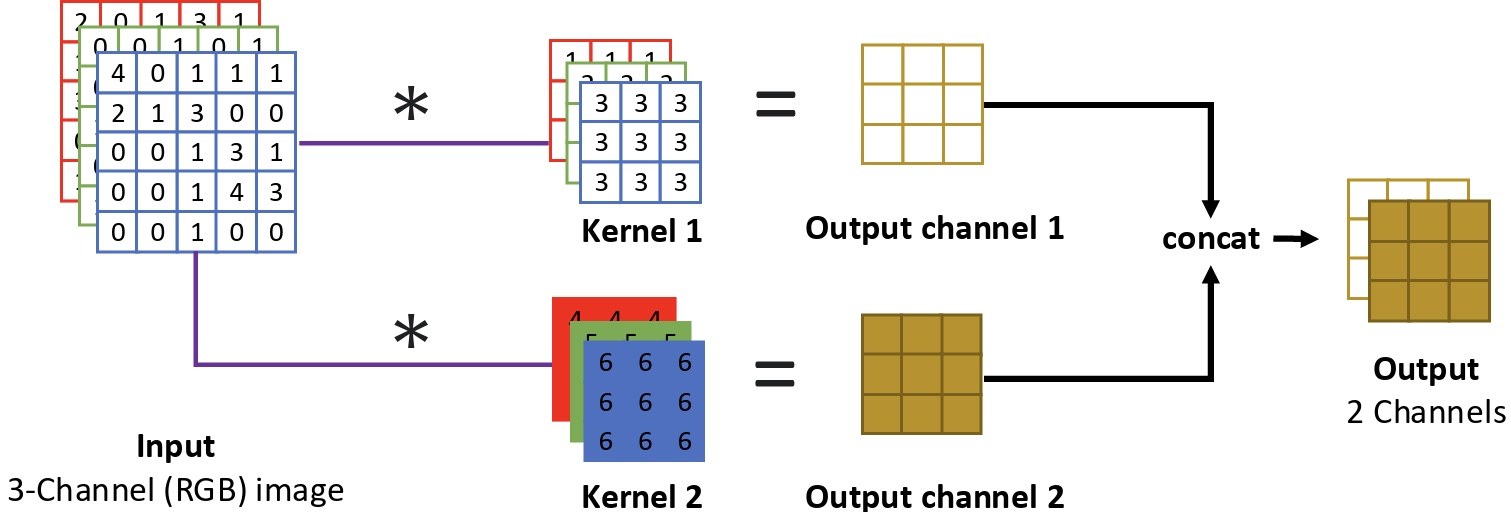
\includegraphics[
      width=\columnwidth,
      trim=0 0 0 0,
      clip
    ]{conv.jpg}
  }\vspace{-0.6em}
\begin{lstlisting}
conv_layer = torch.nn.Conv2d(in_channels=3,out_channels=2,
                    kernel_size=3,stride=1,padding=0)
\end{lstlisting}\vspace{-0.6em}\vspace{-0.6em}
\begin{itemize}
    \setlength{\itemsep}{0pt}
    \setlength{\parskip}{0pt}
    \item \textbf{Vanishing gradient}\vspace{-0.6em}
      \begin{itemize}
        \setlength{\itemsep}{0pt}
        \setlength{\parskip}{0pt}
        \item Small gradients get repeatedly multiplied → approach zero
        \item Mitigation: change activation functions (e.g.\ use ReLU variants)
      \end{itemize}
    \item \textbf{Exploding gradient}\vspace{-0.6em}
      \begin{itemize}
        \setlength{\itemsep}{0pt}
        \setlength{\parskip}{0pt}
        \item Large gradients get repeatedly multiplied → overflow
        \item Mitigation: gradient clipping (clip gradients to \([-c, c]\))
      \end{itemize}
    \item \textbf{Dropout}\vspace{-0.6em}
      \begin{itemize}
        \setlength{\itemsep}{0pt}
        \setlength{\parskip}{0pt}
        \item Randomly zero out activations during training
        \item Mitigates overfitting by preventing co‐adaptation of neurons
      \end{itemize}
    \item \textbf{Early stopping}\vspace{-0.6em}
      \begin{itemize}
        \setlength{\itemsep}{0pt}
        \setlength{\parskip}{0pt}
        \item Monitor validation loss and stop when it ceases to improve
        \item Prevents overfitting by halting before the model fits noise
      \end{itemize}\vspace{-0.6em}
  \end{itemize}\vspace{-0.6em}
  
\textbf{RNN:}\vspace{-0.6em}
\begin{itemize}
    \setlength{\itemsep}{0pt}
    \setlength{\parskip}{0pt}
    \item \textbf{Capture contextual information} — RNNs can aggregate information over the sequence.
    \item \textbf{Sequential dependency} — the prediction at time step \(t\) must wait until all previous steps have been completed (not parallelism-friendly).
  \end{itemize}  \vspace{-0.6em}
One-to-Many: $T_x = 1, T_y > 1$\\
\noindent\makebox[\columnwidth][c]{%
    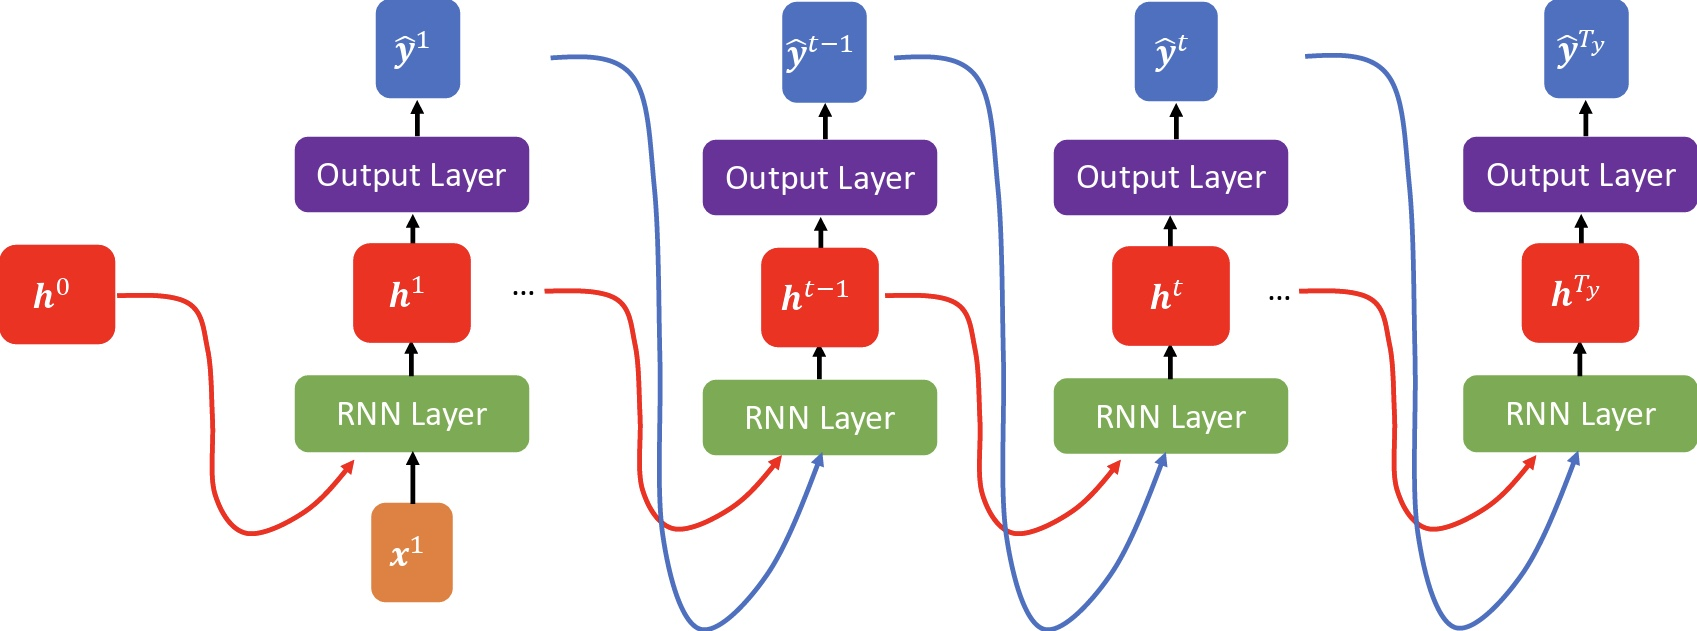
\includegraphics[
      width=\columnwidth,
      trim=0 0 0 0,
      clip
    ]{otm.jpg}
  }
Many-to-One: $T_x = > 1, T_y = 1$\\
  \noindent\makebox[\columnwidth][c]{%
    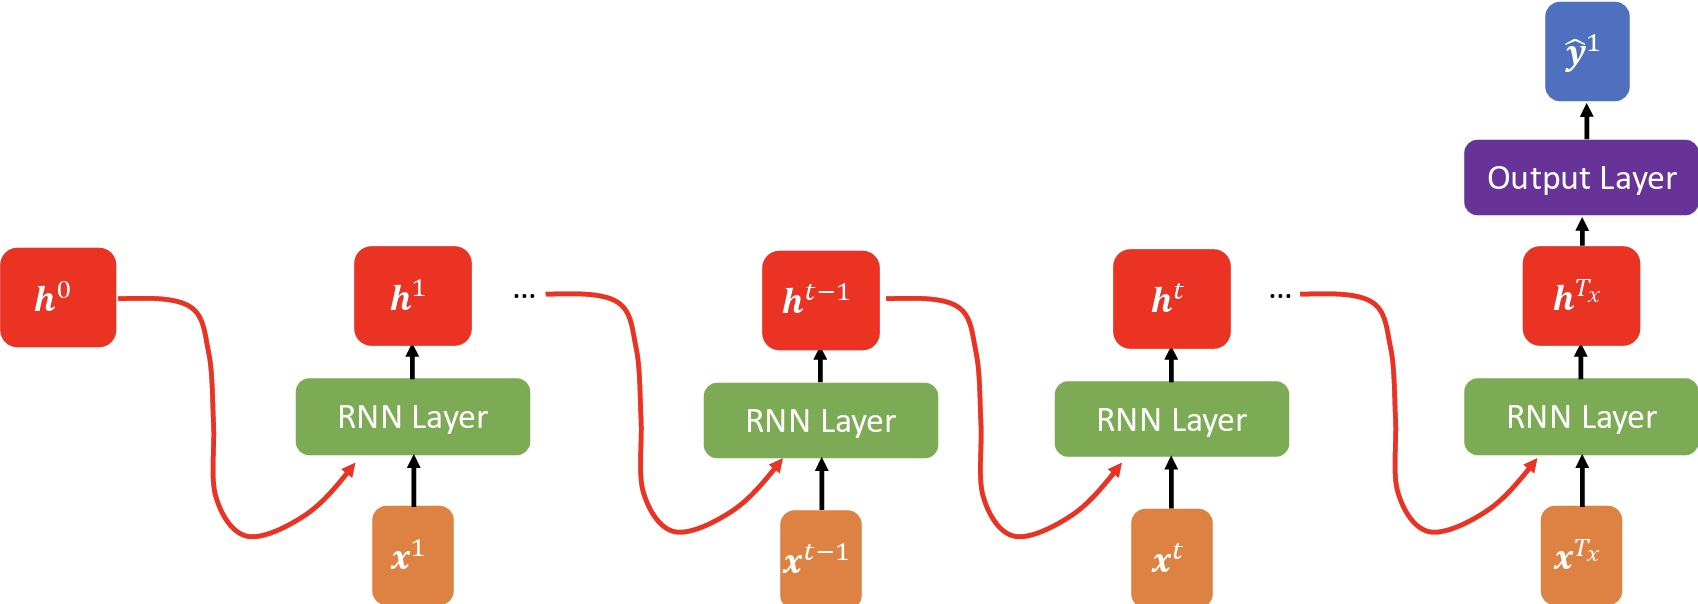
\includegraphics[
      width=\columnwidth,
      trim=0 0 0 0,
      clip
    ]{mto.jpg}
  }
Many-to-Many: $T_x = T_y > 1$\\
  \noindent\makebox[\columnwidth][c]{%
    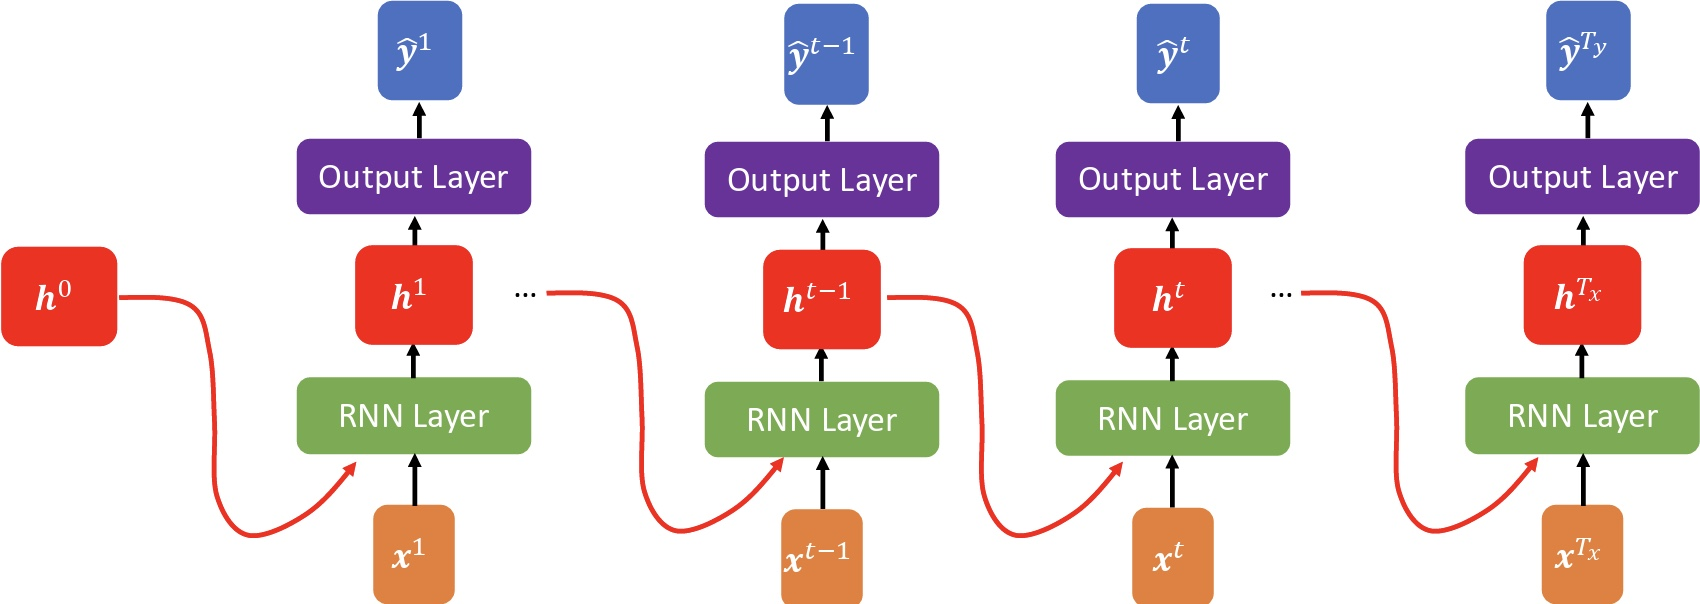
\includegraphics[
      width=\columnwidth,
      trim=0 0 0 0,
      clip
    ]{mtm.jpg}
  }
Many-to-Many: $T_x \neq T_y, T_x > 1, T_y > 1$\\
  \noindent\makebox[\columnwidth][c]{%
    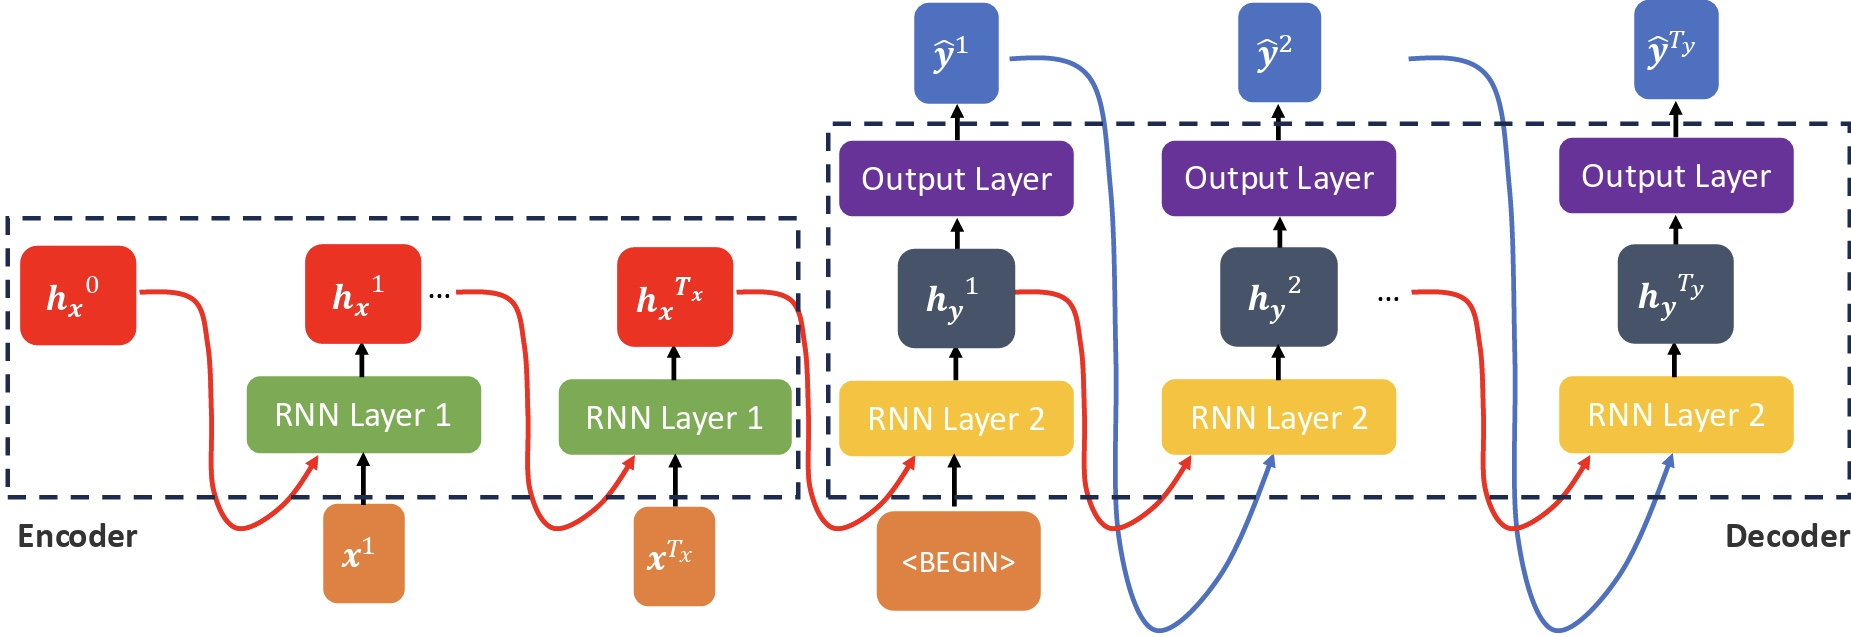
\includegraphics[
      width=\columnwidth,
      trim=0 0 0 0,
      clip
    ]{mtmd.jpg}
  }
\textbf{Attention:}
\[
s_{ij} \;=\; \mathrm{score}(x_i, x_j)
\;=\;\frac{(W^Q x_i)^\top (W^K x_j)}{\sqrt{d_k}}
\quad\text{(raw attention score)}
\]
\[a_{ij} = \mathbf{k}^j\cdot \mathbf{q}^i = (\mathbf{k}^j)^T \mathbf{q}^i = \frac{e^{s_{ij}}}{\sum_{}^{k} e^{s_{ik}}}\] 
\[
      q_i = W^Q x_i,\quad
      k_j = W^K x_j,\quad
      v_j = W^V x_j
    \]
\textbf{Self-Attention Layer:}\\
\noindent\makebox[\columnwidth][c]{%
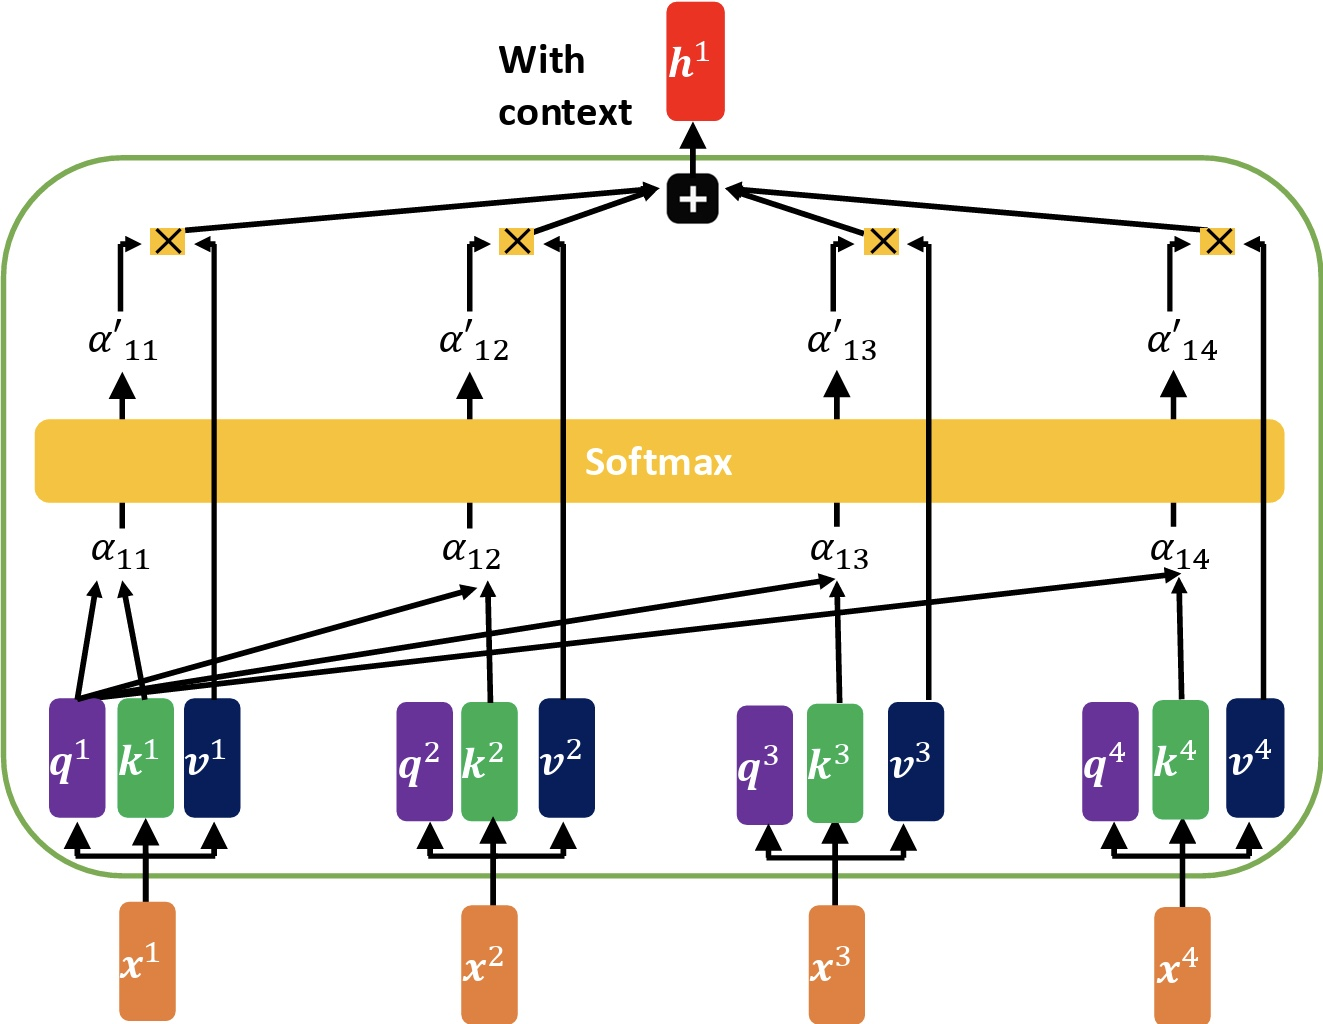
\includegraphics[
  width=\columnwidth,
  trim=0 0 0 0,
  clip
]{slfatt.jpg}
}

% \resizebox{\linewidth}{!}{
% \begin{tikzpicture}[
%     >=Stealth,
%     node distance=2cm and 2.5cm,
%     every node/.style={
%       draw,
%       align=center,
%       minimum width=2.5cm,
%       inner sep=4pt
%     }
%   ]
%   % Nodes
%   \node (dLy) {$\displaystyle \frac{dL}{d\hat y}$\\[2pt] $\hat y - y$};
%   \node[right=of dLy] (dLz3) {$\displaystyle \frac{dL}{dz_3}$\\[2pt] $(\hat y - y)\,g'(z_3)$};
%   \node[right=of dLz3, yshift=10mm] (dLa1) {$\displaystyle \frac{dL}{da_1}$\\[2pt] $(\hat y - y)\,g'(z_3)\,w_5$};
%   \node[right=of dLz3, yshift=-10mm] (dLa2) {$\displaystyle \frac{dL}{da_2}$\\[2pt] $(\hat y - y)\,g'(z_3)\,w_6$};
%   \node[right=of dLa1] (dLz1) {$\displaystyle \frac{dL}{dz_1}$\\[2pt] $(\hat y - y)\,g'(z_3)\,w_5\,g'(z_1)$};
%   \node[right=of dLa2] (dLz2) {$\displaystyle \frac{dL}{dz_2}$\\[2pt] $(\hat y - y)\,g'(z_3)\,w_6\,g'(z_2)$};
%   \node[right=of dLz1] (dLx1) {$\displaystyle \frac{dL}{dx_1}$\\[2pt]
%     $(\hat y - y)\bigl[g'(z_3)\,w_5\,g'(z_1)\,w_1$\\
%     $\quad+\,g'(z_3)\,w_6\,g'(z_2)\,w_2\bigr]$};
%   \node[right=of dLz2] (dLx2) {$\displaystyle \frac{dL}{dx_2}$\\[2pt]
%     $(\hat y - y)\bigl[g'(z_3)\,w_5\,g'(z_1)\,w_3$\\
%     $\quad+\,g'(z_3)\,w_6\,g'(z_2)\,w_4\bigr]$};

%   % Edges
%   \draw[->] (dLy)   -- node[midway,above] {$g'(z_3)$} (dLz3);
%   \draw[->] (dLz3)  -- node[midway,above] {$w_5$}        (dLa1);
%   \draw[->] (dLz3)  -- node[midway,below] {$w_6$}        (dLa2);
%   \draw[->] (dLa1)  -- node[midway,above] {$g'(z_1)$}     (dLz1);
%   \draw[->] (dLa2)  -- node[midway,below] {$g'(z_2)$}     (dLz2);
%   \draw[->, gray] (dLz1) -- node[midway,above] {$w_1$}    (dLx1);
%   \draw[->, blue] (dLz1) -- node[midway,below] {$w_3$}    (dLx2);
%   \draw[->, gray] (dLz2) -- node[midway,above] {$w_2$}    (dLx1);
%   \draw[->, black] (dLz2) -- node[midway,below] {$w_4$}   (dLx2);
% \end{tikzpicture}}
\begin{itemize}
    \setlength{\itemsep}{0pt}
    \setlength{\parskip}{0pt}
  \item \textbf{Raw scores}  
    \[
      s_{ij} = q_i^\top k_j = (k_j)^\top q_i
    \]  
  \item \textbf{Attention weights (softmax)}  
    $
      a_{ij} = \frac{\exp(e_{ij})}{\sum_{l}\exp(e_{il})}
    $  
  \item \textbf{Positional encoding}  
    \[
      x'_i = x_i + PE_i,
      \quad
      PE_{i,2k}   = \sin \bigl(i/10000^{2k/d}\bigr),
      \quad\]\[
      PE_{i,2k+1} = \cos \bigl(i/10000^{2k/d}\bigr)
    \]  
\end{itemize}
\begin{itemize}
    \setlength{\itemsep}{0pt}
    \setlength{\parskip}{0pt}
    \item Attention Neural Networks
    \begin{itemize}
        \setlength{\itemsep}{0pt}
        \setlength{\parskip}{0pt}
        \item Masked Self-Attention
        Linear projections to queries/keys/values, scaled dot-product with causal mask to prevent “seeing” future tokens.
        \item Cross-Attention
        Same mechanism, but queries from decoder attend over encoder’s key/value projections.
        \item Transformer Architecture
        Stacks of encoder/decoder blocks combining (masked) self-attention, cross-attention, and feed-forward sublayers.
    \end{itemize}
\end{itemize}
ANN: Many-to-Many: $T_x = T_y > 1$\\
\noindent\makebox[\columnwidth][c]{%
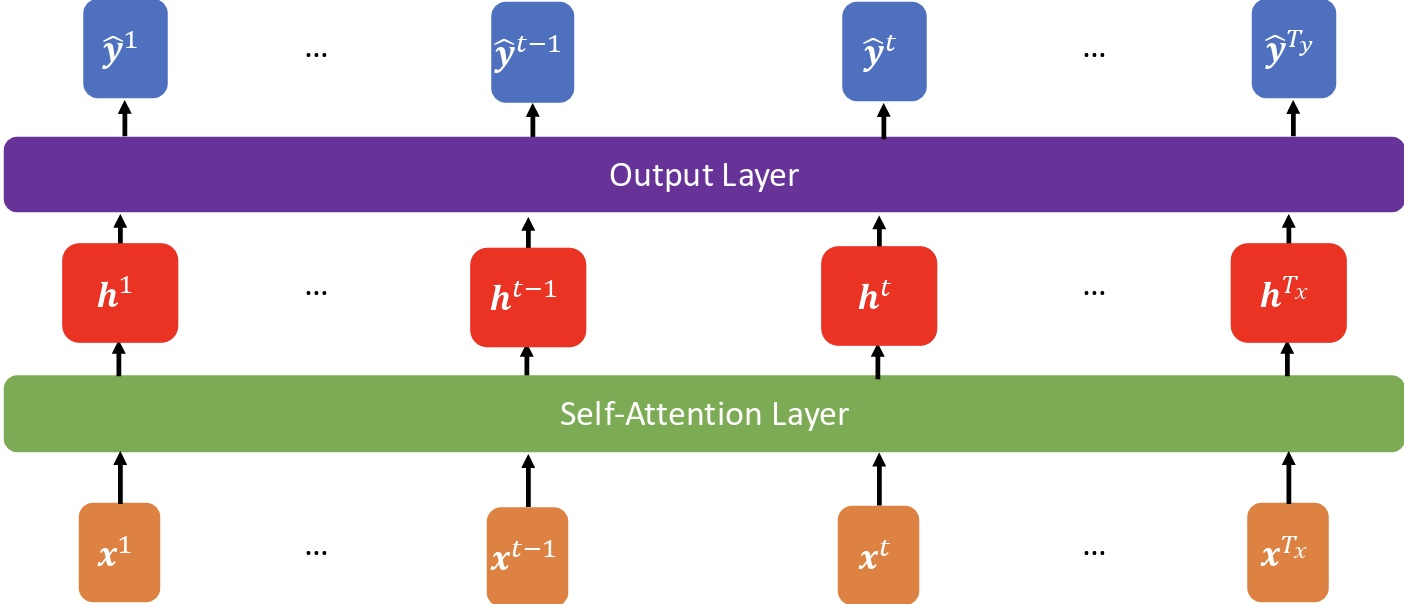
\includegraphics[
  width=\columnwidth,
  trim=0 0 0 0,
  clip
]{atmtm.jpg}
}
Many-to-One: $T_x > 1, T_y = 1$; One-to-Many: $T_x = 1, T_y > 1$\\
\noindent\makebox[\columnwidth][c]{%
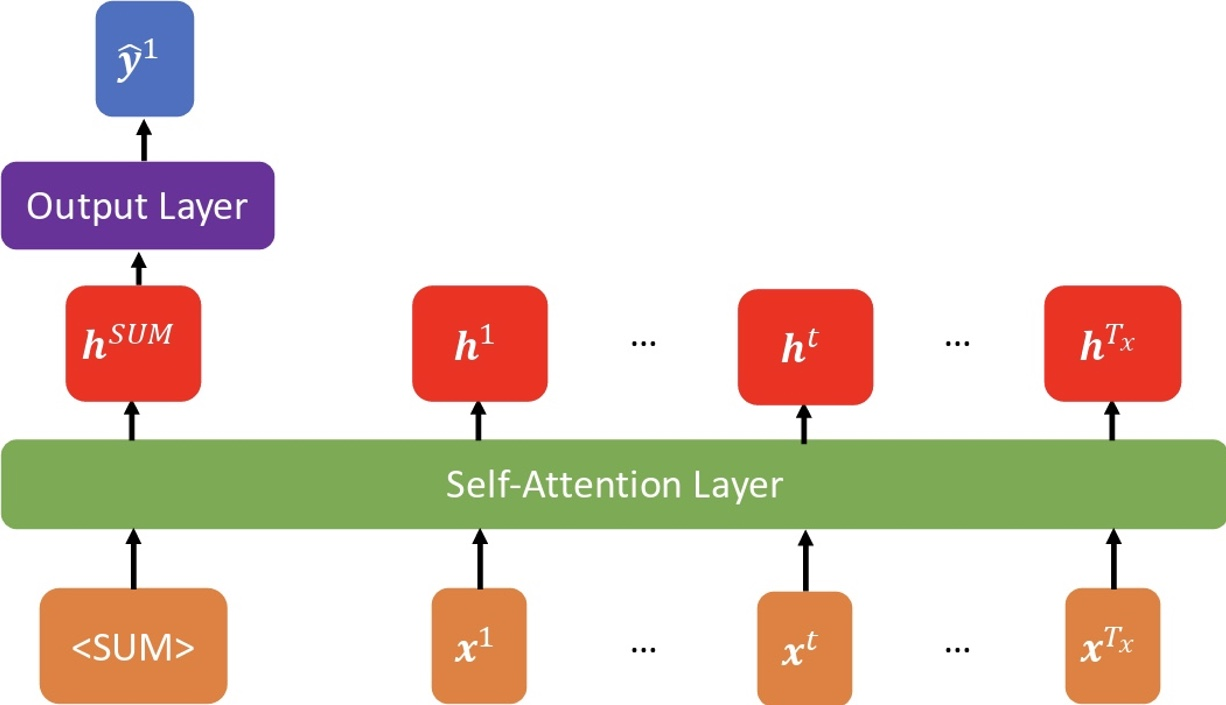
\includegraphics[
  width=\columnwidth,
  trim=0 0 0 0,
  clip
]{atmto.jpg}
}

\noindent\makebox[\columnwidth][c]{%
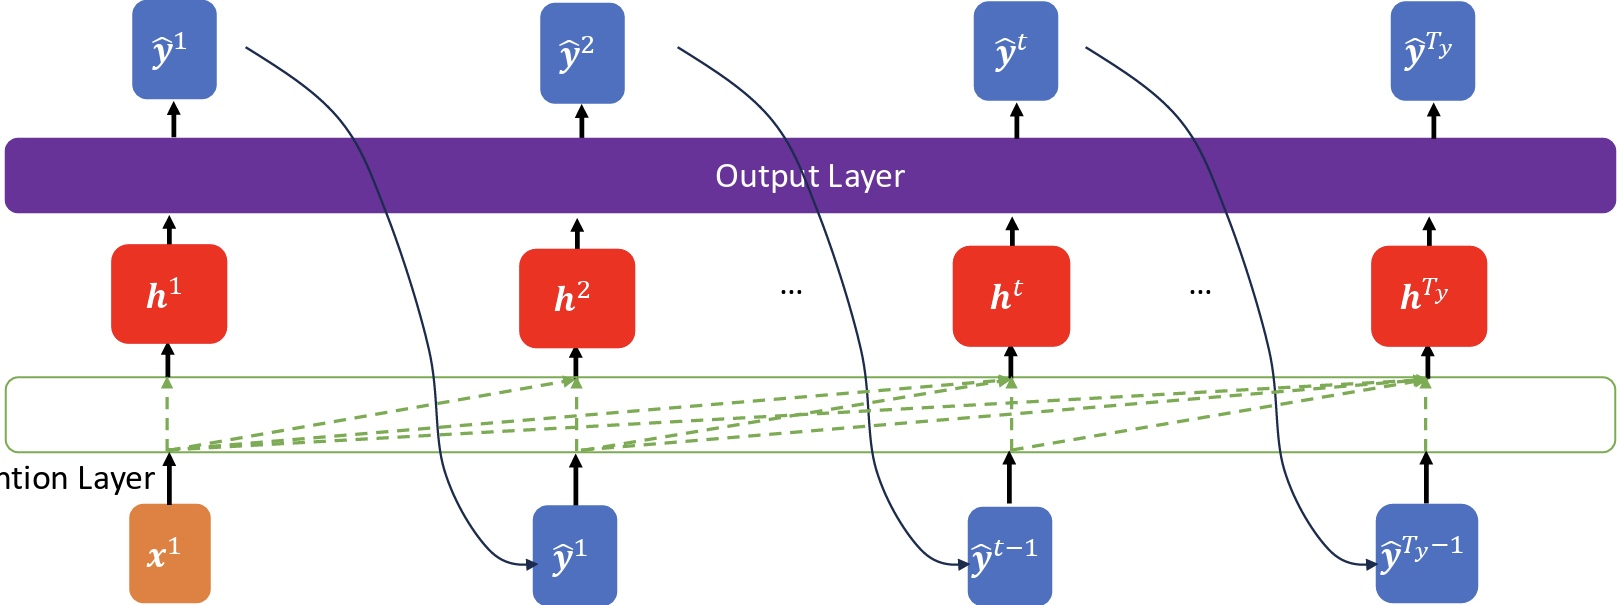
\includegraphics[
  width=\columnwidth,
  trim=0 0 0 0,
  clip
]{atotm.jpg}
}
\noindent\makebox[\columnwidth][c]{%
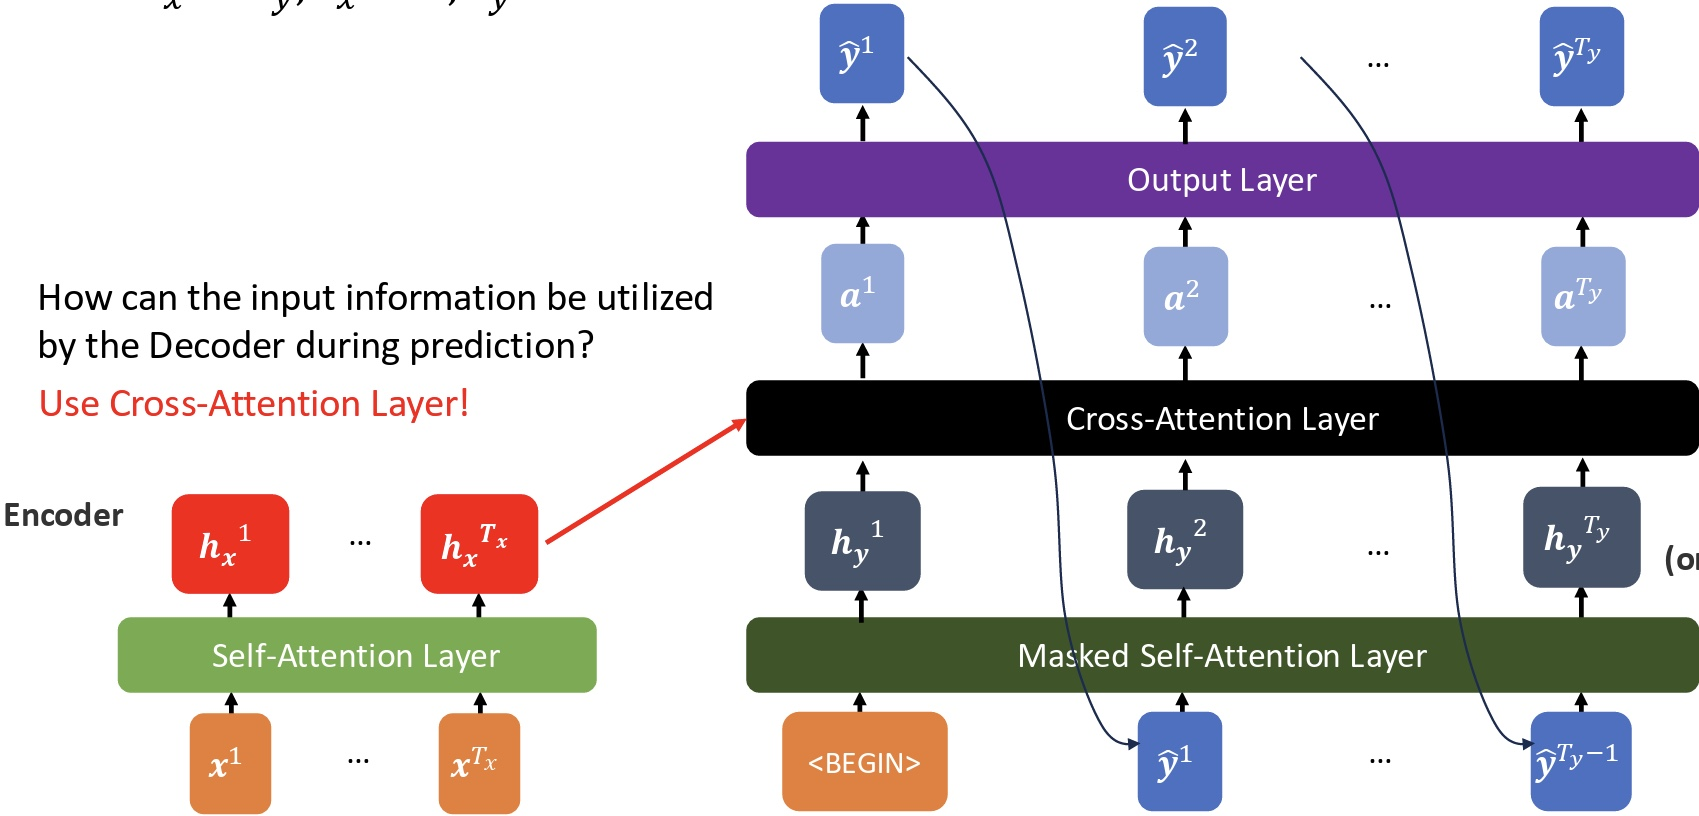
\includegraphics[
  width=\columnwidth,
  trim=0 0 0 0,
  clip
]{atnmtm.jpg}
}
\noindent\makebox[\columnwidth][c]{%
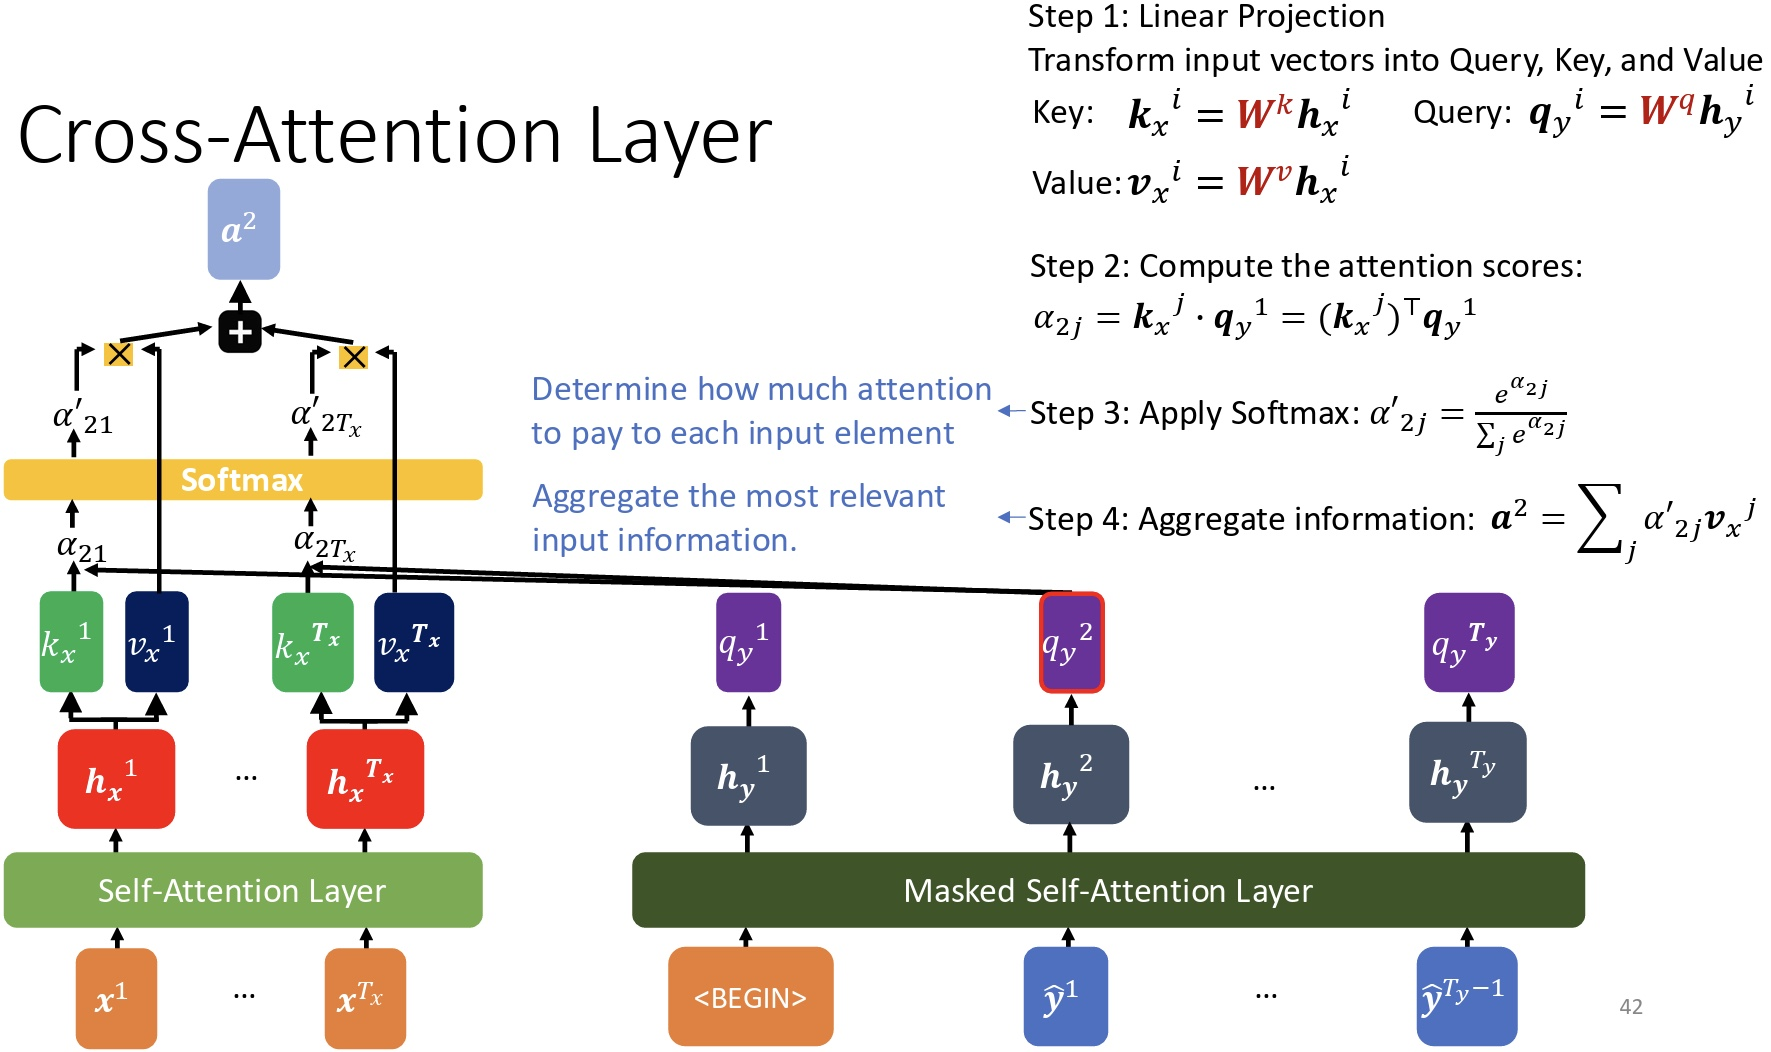
\includegraphics[
  width=\columnwidth,
  trim=0 0 0 0,
  clip
]{catl.jpg}
}
\textbf{Transformer:}\\
\noindent\makebox[\columnwidth][c]{%
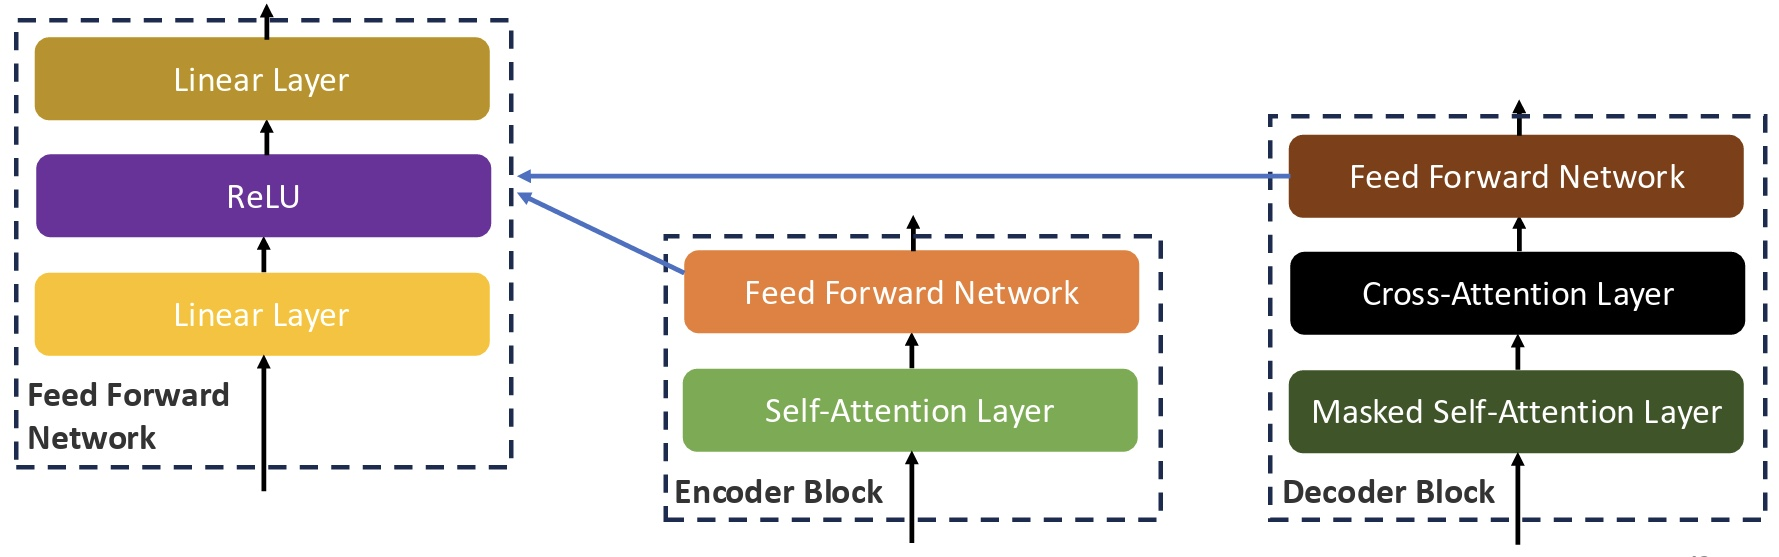
\includegraphics[
  width=\columnwidth,
  trim=0 0 0 0,
  clip
]{tfm.jpg}
}
\end{document}

